\documentclass[preview, border=1mm]{standalone}
\usepackage{tikz}
\usetikzlibrary{automata, positioning}

% Sample document state diagram.
% NFSA from Tutorial Worksheet 1, Question 5(a)
\begin{document}
  \vspace*{1cm}
  \hspace*{1cm}
  % This resize box helps with padding around the image.
  \resizebox{0.8\linewidth}{!}{
    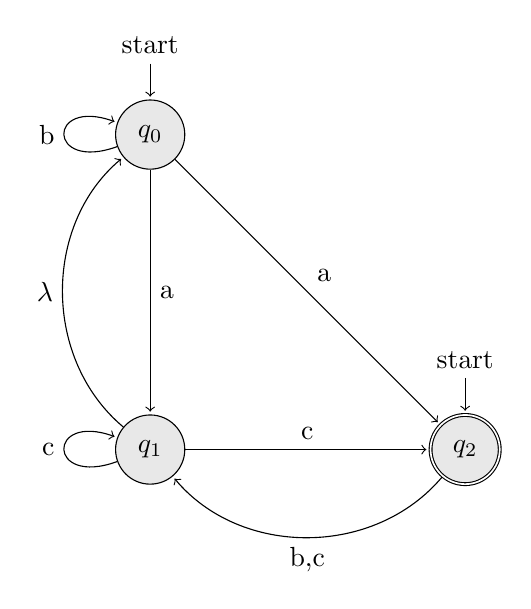
\begin{tikzpicture}[shorten >= 1pt, node distance=2cm,auto]
      \tikzstyle{every state}=[fill={rgb:black, 1; white, 10}]

      % Initialise each node and set its position.
      \node[state, initial above]
        (q_0) at (0,0)    % q_0 position is top left.
        {$q_0$};s
      \node[state]
        (q_1) at (0,-4)   % q_1 position is bottom left.
        {$q_1$};
      \node[state, initial above, accepting]
        (q_2) at (4,-4)   % q_2 position is bottom right.
        {$q_2$};

      % Draw the paths with edges labeled.
      \path[->]
        (q_0)
          edge node {a} (q_1)
          edge node {a} (q_2)
          edge[in=160, out=200, loop] node[left] {b} (q_0)
        (q_1)
          edge[bend left=50] node[left] {$\lambda$} (q_0)
          edge[in=160, out=200, loop] node[left] {c} (q_1)
          edge node {c} (q_2)
        (q_2)
          edge[bend left=50] node[below] {b,c} (q_1);
    \end{tikzpicture}
  }
  \hspace{1cm}
  \vspace{1cm}
\end{document}